Here we compare the performance of each voting algorithm with respect to the average happiness achieved by the elected candidate and
the effect of opinion transparency. \newline
\indent In Figure~\ref{fig:satisfaction_hists}, we show for varying threshold values the distributions of satisfaction for each
voting algorithm. This demonstrates the efficacy of each voting scheme with respect to satisfaction. We see that plurality
is shown to have the minimum happiness in all three scenarios with approval based voting tending towards a higher mean.
Although the differences in mean happiness are slight, we believe that the fact that these distributions are realized over
100 separate simulations indicates that indeed approval-based and ranked-choice voting seek a more optimal candidate solution
than plurality.
\begin{figure}[h!]
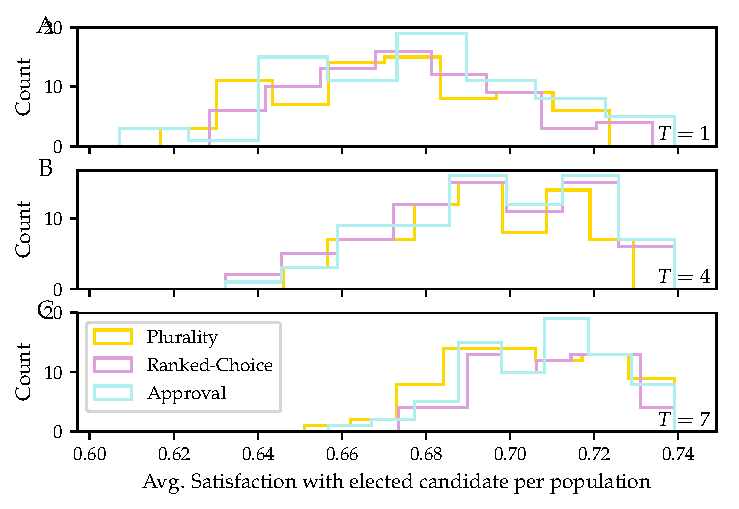
\includegraphics[width=0.5\textwidth]{../src/figs/new/satisfaction-hist_avgperpop.pdf}
\caption{Average Happiness for all populations for each voting system and transparency level}
\label{fig:satisfaction_hists}
    \caption{Histograms of the average satisfaction/happiness/agreement of the populations with the elected
    candidate. Each panel represents the a simulation for opinion transparency levels $T$ found
    in the bottom right corner. }
\end{figure}
The notion of the plurality method's ill-performing nature in finding the most utilitarian candidate
is further indicated by visualizing voter satisfaction as a function of opinion transparency in Figure~\ref{fig:avghapp_by_transparency}.
Here we see that plurality clearly performs the worst among the three, barely overlapping in standard error with the latter two.
Meanwhile, ranked-choice and approval-based voting show a higher trend.
\begin{figure}[h!]
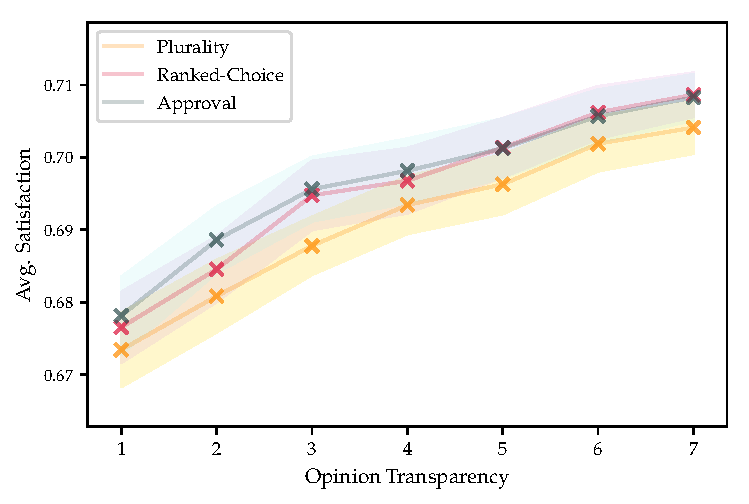
\includegraphics[width=0.5\textwidth]{../src/figs/new/avghapp_transparency.pdf}
\caption{Average citizen satisfaction for all populations for each voting system and transparency level shown
    with 95\% confidence interval of standard error.}
\label{fig:avghapp_by_transparency}
\end{figure}
